\documentclass[aspectratio=169]{beamer}

\usetheme{default}
\setbeamertemplate{navigation symbols}{}

\usepackage{graphicx}
\usepackage{booktabs}

\title{Rotation and Composition Findings}
\author{}
\date{12 February 2026}

\begin{document}

\begin{frame}
  \titlepage
\end{frame}

\begin{frame}{Questions}
  \begin{itemize}
    \item Is the composed kernel rotation invariant?
    \item Why is composite accuracy lower than regular all-kernel model?
  \end{itemize}
\end{frame}

\begin{frame}{Rotation-Invariance}
  \begin{itemize}
    \item Composition is a weighted sum: $K_{comp}=\sum_i w_i K_i$.
    \item This is not automatically rotation invariant.
    \item Non-rotation-invariant kernel families in the 9-bank: anisotropic Gaussian, Gabor, HOG, LBP, GLCM.
    \item For the analyzed composition run, 90/180/270$^\circ$ checks show large differences.
    \item \textbf{Current composite kernel is not rotation invariant. But...}
  \end{itemize}
\end{frame}

\begin{frame}{Non-Invariant But Still Robust}
  \begin{itemize}
    \item 90$^\circ$/180$^\circ$ test rotation still gave stable accuracy:
    \item Regular model: $\Delta$AUC $+0.0017$, $\Delta$ACC $+0.0123$
    \item Composite model: $\Delta$AUC $+0.0086$, $\Delta$ACC $+0.0241$
    \item Takeaway: non-invariant kernels can still yield stable accuracy.
  \end{itemize}
\end{frame}

\begin{frame}{Why Composite is Lower}
  \begin{itemize}
    \item Feature collapse $\rightarrow$ fix: use a small bank of composites (e.g., 8--32) instead of one.
    \item Nonlinearity mismatch with \texttt{abs\_max} $\rightarrow$ fix: make the response linear by replacing \texttt{abs\_max} with linear pooling (mean or sum), so composing kernels before response is closer to combining features after response.
  \end{itemize}
\end{frame}

\begin{frame}{Best Current Run}
  \begin{center}
    \begin{tabular}{lcc}
      \toprule
      Model & Test AUC & Test ACC \\
      \midrule
      Regular (separate kernels) & 0.9376 & 0.8888 \\
      Composite (8 kernels) & 0.9026 & 0.8299 \\
      \bottomrule
    \end{tabular}
  \end{center}
  \vspace{0.5em}
  \small composition remains below separate kernels in this run.
\end{frame}

\begin{frame}{Composite Kernels (Grid)}
  \begin{center}
    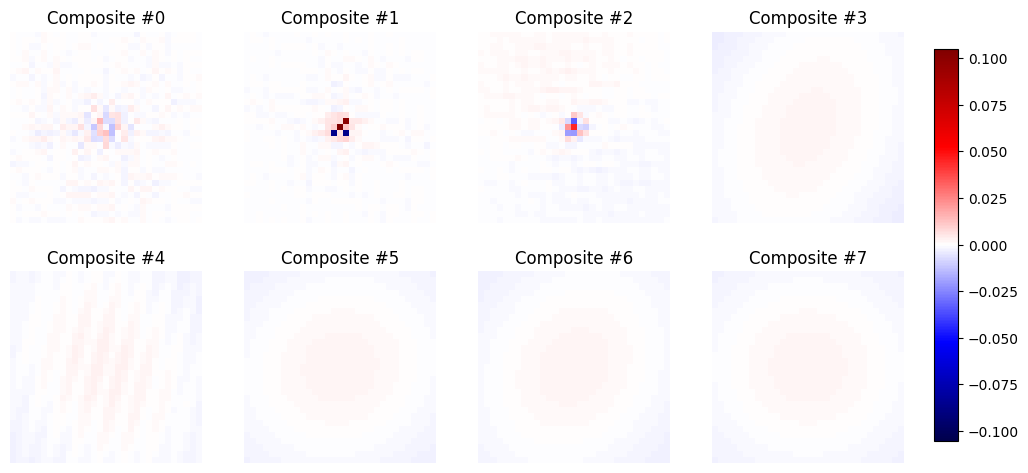
\includegraphics[width=0.95\linewidth]{../../results/exp_022/composite_kernels_grid.png}
  \end{center}
\end{frame}


\begin{frame}{Current Pipeline and Next Step}
  \begin{itemize}
    \item Current: Kernel generation is random.
    \item Change: Smarter sampling using QMC or Latin Hypercube.
    \item Current: normalization is applied to composed kernels; non-composed kernels are used without an extra normalization stage. Prior runs without extra normalization performed better.
    \item Change: test per-family normalization (different normalization per kernel type).
  \end{itemize}
\end{frame}

\begin{frame}{Conclusion}
  \begin{itemize}
    \item Current composite is not rotation invariant.
    \item Composite underperforms regular model mainly due to information compression and nonlinearity effects.
    \item Matching regular accuracy is more realistic with multiple composites than a single one.
    \item Larger composition pools can look ``zoomed'' due to cancellation and normalization.
  \end{itemize}
\end{frame}

\end{document}
